\begingroup
\newcommand{\GerlingSeptSeconds}[2]{#1\makebox[.42em][c]{,\makebox[0pt][r]{\textsuperscript{s}}}#2}
\begin{center}
\textsc{Gauss} an \textsc{Gerling}.\quad Göttingen, 1.~September 1823.
\end{center}

\par\noindent\hspace*{\parindent}\mbox{.\ .\ .\ .\ .\ .\quad Ich} habe Ihnen nur den Modus meines Telegraphirens angezeigt; bestimmte bleibende Werthe haben die Zahlzeichen nicht, ebenso wenig wie \(a\) und \(x,y,z\) in der Algebra; die Bedeutungen werden immer für solche Umstände, als sich eben im voraus erwarten lassen, vorher verabredet.
Ich besorge indess, dass das Telegraphiren wenigstens mit dem Meisner-Heliotrop sehr bedenklich sein würde, denn es scheint mir, dass er sehr unvollkommen berichtigt sein muss.
Besonders in der Stunde von 2---3\textsuperscript{h} (wo doch die übrigen Gegenstände gewöhnlich zu stark wallen, um etwas brauchbares messen zu können)\textsuperscript{*}), habe ich allezeit die Erfahrung gemacht, dass das Licht, wenn es im besten Leuchten ist, plötzlich abgebrochen wird, dann eine Zeit lang ganz unsichtbar bleibt, und dann allmählig äusserst klein anfängt und zuletzt erst den vollen Glanz erhält, aber leider nur kurze Zeit \textls[120]{behält} (manchmal nur \(\frac{1}{4}\) Minute); unter solchen Umständen ist aber an zuverlässiges Telegraphiren nicht zu denken.
\par\smallskip\noindent\rule{.24\linewidth}{.4pt}\par\nobreak
{\footnotesize\noindent\hspace*{\parindent}\textsuperscript{*}) Nemlich zwischen 6 und 7\textsuperscript{h} habe ich es seltener beachtet, weil ich keine Zeit für Messung verlieren wollte.\par}
\smallskip\noindent\hfill{\small49\textsuperscript{*}}\hspace*{.123\linewidth}\par
\clearpage
\noindent\makebox[0pt][l]{\fontsize{13}{16}\selectfont 388}\hfill{\small\textbf{BRIEFWECHSEL MIT GERLING.}}\hfill\null\par\medskip
\par\noindent\hspace*{\parindent}Ich habe 1822 einen ähnlichen Fall mit dem damals auf dem Deister befindlichen ältesten Heliotrop gehabt, dessen Rectification vermuthlich durch unsanften Transport gelitten hatte.
Ich half damals durch ein Palliativmittel.
Es wurden nemlich öfters Versuche gemacht, indem ich zuerst dem Lieutenant \textsc{Hartmann} durch ein bestimmtes Zeichen andeutete, \textls[120]{dass} die Versuche gemacht werden sollten.
Dann liess er das Sonnenbild zu oft wiederholten Malen in verschiedenen Höhen durch das Fadenkreuz gehen,
\par\vspace{.7cm}
{\centering
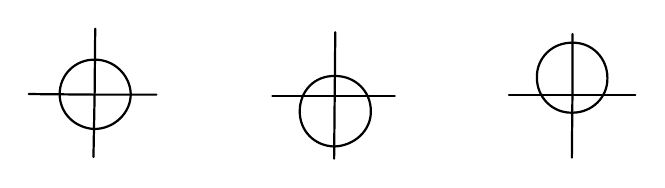
\begin{tikzpicture}[x=.0074cm,y=-.0074cm,line width=.8pt,line cap=round,line join=round]
\draw (103,151) .. controls (103,118) and (130,91) .. (164,92) .. controls (197,92) and (224,119) .. (225,151) .. controls (225,184) and (196,211) .. (162,211) .. controls (129,209) and (103,184) .. (103,151) -- cycle;
\draw (50,151)--(163,152)--(269,152);
\draw (164,39)--(163,151)--(161,259);
\draw (515,181) .. controls (515,146) and (540,119) .. (576,120) .. controls (610,120) and (637,146) .. (637,180) .. controls (638,213) and (609,240) .. (574,241) .. controls (540,240) and (515,214) .. (515,181) -- cycle;
\draw (468,154)--(575,154)--(678,154);
\draw (576,45)--(575,154)--(574,262);
\draw (922,123) .. controls (921,89) and (949,62) .. (983,63) .. controls (1017,62) and (1043,90) .. (1043,123) .. controls (1044,157) and (1016,183) .. (983,183) .. controls (949,184) and (922,157) .. (922,123) -- cycle;
\draw (874,153)--(983,153)--(1091,153);
\draw (983,48)--(983,153)--(982,260);
\end{tikzpicture}\par}
\vspace{.7cm}\noindent und ich zeigte ihm den Augenblick, wo ich sein volles Licht zuerst sah, durch Eröffnung meines Heliotrops, und den Schluss des vollen Lichts durch Bedeckung an.
Es versteht sich, dass dabei mein Heliotrop immer beinahe central die Sonne auf dem Fadenkreuz hatte, um ganz gewiss zu sein, dass mein Licht völlig hinkomme.
Meinerseits waren also 3 Personen nöthig: Einer, der immer den Heliotrop fast central unterhielt, ein Zweiter, der mit dem Fernrohr (die Distanz war \(8\frac{1}{2}\) Meilen) den jenseitigen Heliotrop beobachtete und ein Dritter, der auf des Zweiten Zurufen den Spiegel des Heliotrops öffnete oder bedeckte (bloss durch Vortreten mit seinem Körper).
Ich wollte dies recht gern auch mit Ihnen thun.
Das 3-fache Attentionszeichen (\GerlingSeptSeconds{1}{2} zu, \GerlingSeptSeconds{1}{2} offen, \GerlingSeptSeconds{1}{2} zu, etc.\ etc.) könnte die Intention des Versuchs andeuten (den man immer nur macht, wenn wenig Gefahr von Wolkenbedeckung stattfindet), und zwar gibt der das Zeichen zuerst, der den Heliotrop des andern prüfen will.
Da Gelehrten gut predigen ist, so brauche ich wohl nichts über die Benutzung der Versuche beizufügen.
Bei ähnlicher Winkelstellung ist dies Mittel fast so gut wie wirkliche Berichtigung, da derjenige, der den geprüften Heliotrop hat, weiss, wie er das Sonnenbild durchgehen lassen muss, und ob er umstellen muss, \textls[120]{ehe} die Sonne ausgetreten ist, oder nachdem sie schon ein Stück ausgetreten, etc.
Bei dem \textls[120]{neuen} Heliotrop wird hoffentlich die Berichtigung gut sein.
\par\noindent\hspace*{\parindent}Was Sie mir von dem \textls[120]{Unterschiede} Ihres Zeichengebens mit dem meinigen schreiben, ist mir nicht ganz deutlich.
Etwas durchaus wesentliches
\par\clearpage
\noindent\null\hfill{\small\textbf{ZUR HANNOVERSCHEN TRIANGULATION.}}\hfill\makebox[0pt][r]{\fontsize{13}{16}\selectfont 389}\par\medskip
\noindent scheint mir zu sein, dass das Attentionszeichen nothwendig erst \textls[120]{erwiedert} sein muss, ehe das wirkliche Zeichen gegeben wird, ob aber jenes und dieses Zeichen mit einem besondern Fernrohr oder in Ermangelung eines solchen mit dem Heliotropfernrohr beobachtet wird, ist wohl eines und dasselbe.
\par\noindent\hspace*{\parindent}Der Modus meiner Zeichen ist von mir öfters verändert, derjenige, den ich Ihnen geschrieben, scheint mir der zweckmässigste.
Allein ich habe leider versäumt, mir selbst eine Abschrift zu machen, und erinnere schon jetzt bloss aus dem Gedächtniss mich nicht mehr ganz genau.
Lassen Sie mir also doch gütigst diese Stelle meines Briefes \mbox{copiren.\quad.\ .\ .\ .\ .\ .}
\par
\endgroup
